\documentclass{article}
%Preamble
\usepackage{float}
\usepackage{color}
\usepackage{listings}
\usepackage{longtable}
\usepackage{amsmath,amssymb}
\usepackage{graphics}
\usepackage{graphicx}

\title{AE 706 -Computational Fluid Dynamics \\ Assignment 2: Report \\ Solution to Laplace Equation using Jacobi, Gauss Siedel and Successive Over Relaxation Method}
\author{Aditi Taneja}
\date{\today}

\begin{document}
\pagenumbering{arabic}
\maketitle

\textbf{Consider a unit square with the bottom left corner at the origin. Discretize the square into an N x N grid. Set the boundary conditions to $x^2 - y^2$. \\ Implement the Jacobi, Gauss-Seidel, and SOR schemes. At each iteration, calculate the difference between the previous solution and the next i.e.}
\\

$err= \frac{\sqrt{\sum_{i=1}^{n}\sum_{j=1}^{n}{(\phi^{n+1}_{i,j} - \phi^{n}_{i,j})^2}}}{N}$
 \\
\textbf{Also calculate the residue instead of the error above and see how that behaves. Iterate until the difference  is less than the machine epsilon*2. \\}
\newpage
\textbf{$1.$ Solve this problem for N=11, 21, 41, and 101. Plot the error versus the iteration count on a semilog plot. Do this for the Jacobi and Gauss-Seidel schemes. }

\begin{figure}[H] \label{figure}
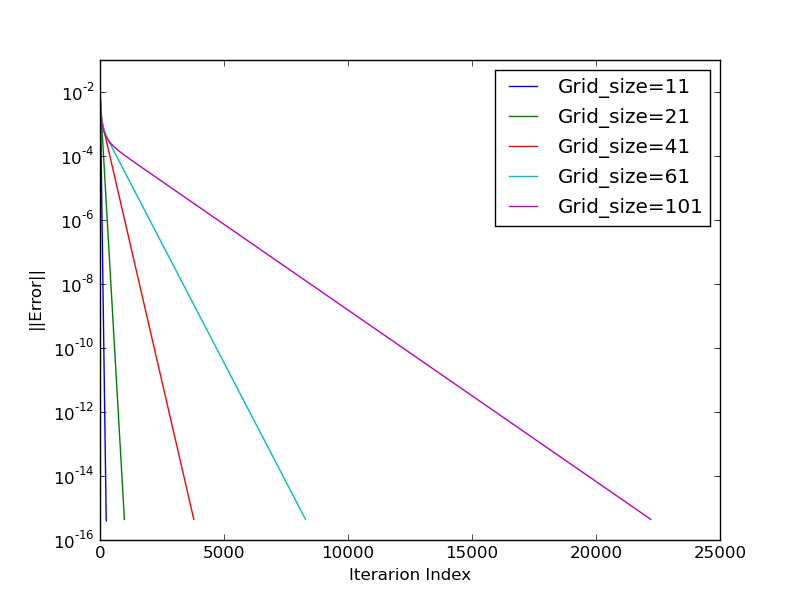
\includegraphics[width=8cm]{jacobi.png}
\label{figure:}
\caption{Plot of the norm of error versus iteration for the solution to Laplace’s equation using the Jacobi method for various grid sizes}
\end{figure}

\begin{figure}[H] \label{figure}
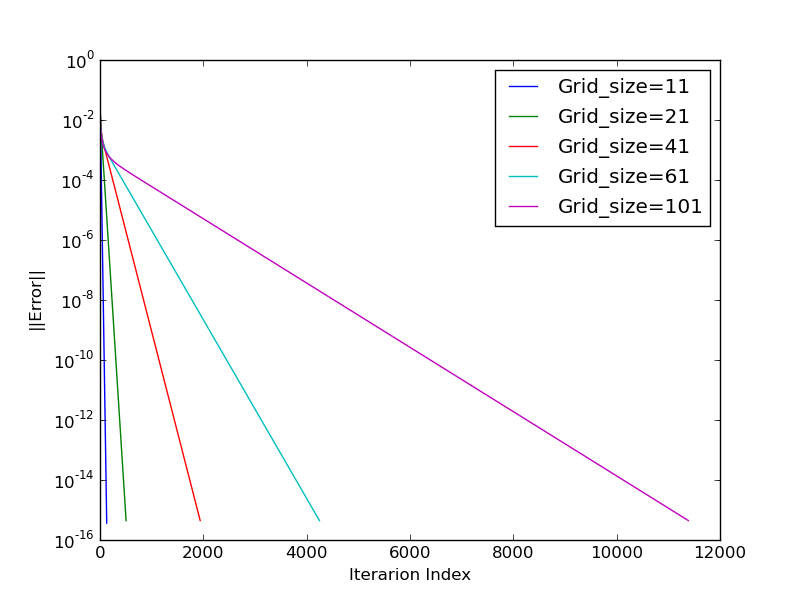
\includegraphics[width=8cm]{gs.png}
\label{figure:}
\caption{Plot of the norm of error versus iteration for the solution to Laplace’s equation using the Gauss Siedel method for various grid sizes}
\end{figure}

\begin{figure}[H] \label{figure}
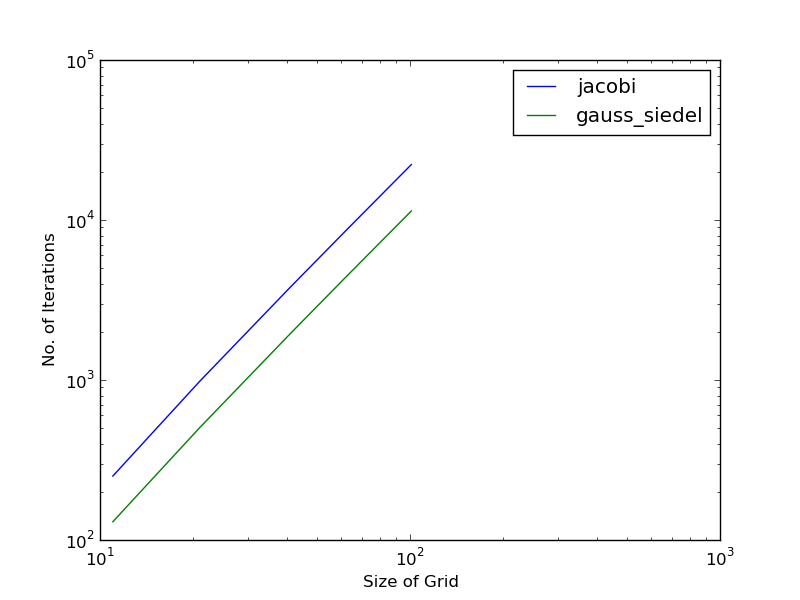
\includegraphics[width=10cm]{ex_1.png}
\caption{Number of Iterations to convergence vs. Grid size for Jacobi and Gauss Siedel Method}
\label{figure:}
\end{figure}

\begin{description}
\item[]Figure 1. and Figure 2. shows that as size of grid increases number of iterations to converge to 2*machine\_epsilon increases. This is because with increase in grid size, number of computations increase per step for both Gauss Siedel and Jacobi Methods.

\item[]Figure 3. shows that Gauss Siedel method converges faster that jacobi method for same grid size. This is because Gauss siedel method uses values from the same iteration to update the matrix, while Jacobi method uses values from the previous iteration. Gauss Siedel is usually twice as fast as Jacobi method as evident from Figure 15. 
\end{description}

\newpage
\textbf{2. For the SOR scheme, choose N=41. Fix the number of iterations to 20 and hunt for a suitable w value between 0 to 2 in steps of 0.1.}
\begin{figure}[H] \label{figure}
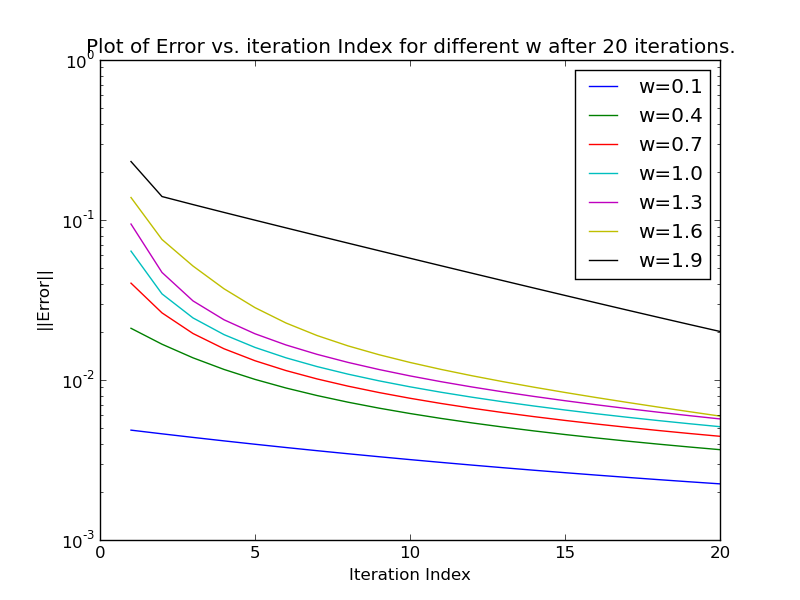
\includegraphics[width=10cm]{all_w_41_20_10.png}
\caption{Plot of norm of error vs. number of iterations for different w in SOR scheme for a 41x41 grid.}
\label{figure:}
\end{figure}

\begin{figure}[H] \label{figure}
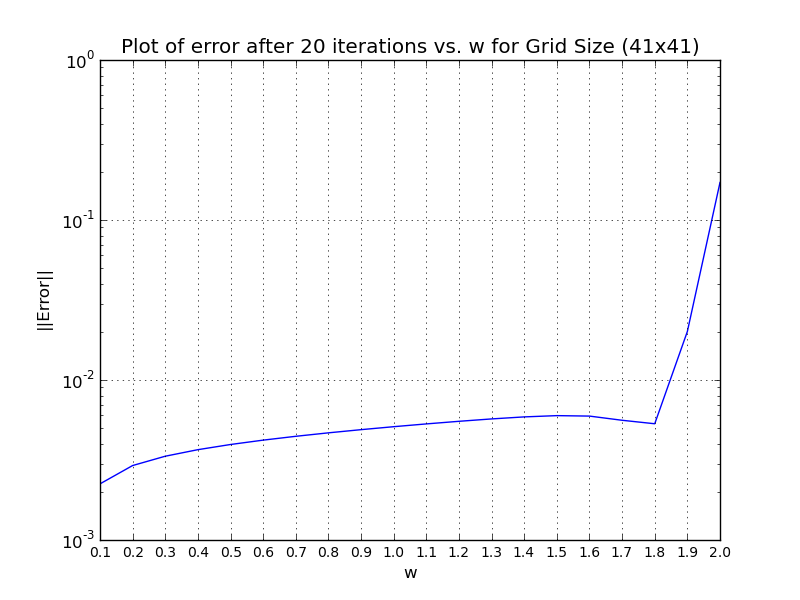
\includegraphics[width=10cm]{w_41_20_10.png}
\caption{Plot of norm of error at the end of 20 iterations vs. w in SOR scheme for a 41x41 grid.}
\label{figure:}
\end{figure}

\begin{figure}[H] \label{figure}
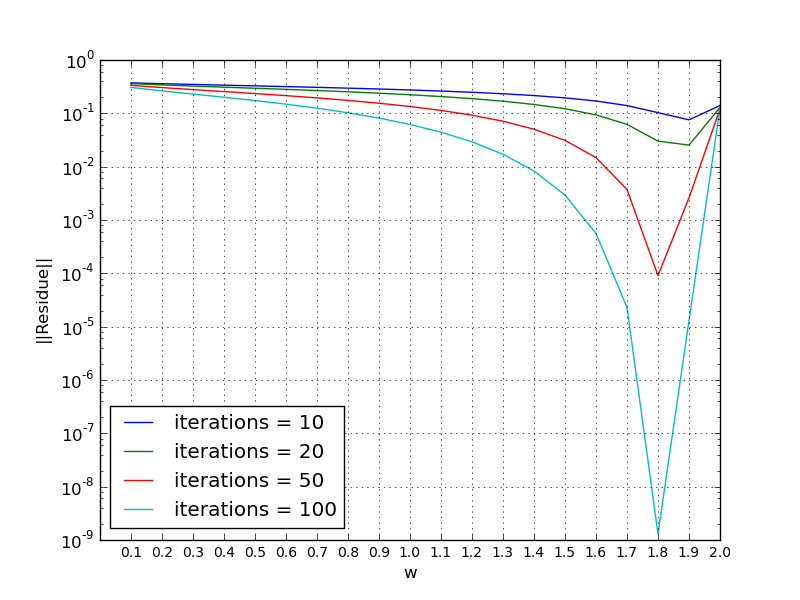
\includegraphics[width=10cm]{residue_41.png}
\caption{Plot of residue at the end of 10,20,50,100 iterations vs. w in SOR scheme for a 41x41 grid.}
\label{figure:}
\end{figure}

\begin{description}
\item[]From the error plot, it is evident that error increases first, and then starts decreasing and then again increasing around 1.8 but the minimum error for 20 iterations on a 41x41 grid occurs at 0.1.
\item[]However from the norm of residue vs. w plot, it can been seen that error decreases till around 1.8, attains a minimum value and then increases suddenly.
\item[]The difference in error and residue trend occurs because error is calculated by using difference between two consecutive iterations, which may be small initially, but residue is calculated by difference between exact function and approxiamte function for that iterations which will be high initially. Therefore, for small number of iterations, while residue continuously decreases, error may increase first and then decrease. Hence mininum values of error and residue may be different for small iterations.
\item[]The value of w should be taken less than but close to 1.8 because there is a steep increase in error/residue after 1.8.
\end{description}

\newpage
\textbf{3. Repeat problem 2 with the number of iterations set to 50 and 100.  Check if the plot changes.}

\begin{figure}[H] \label{figure}
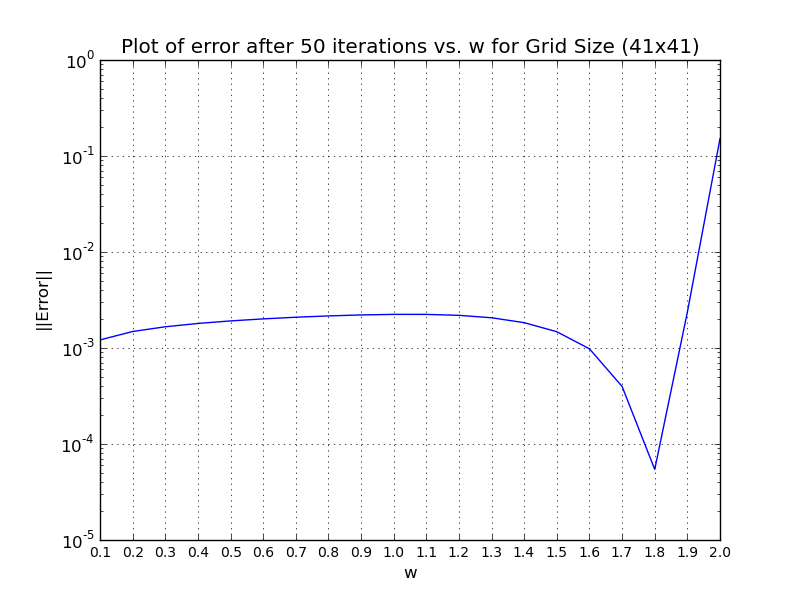
\includegraphics[width=8cm]{w_41_50_10.png}
\caption{Plot of norm of error at the end of 50 iterations vs. w in SOR scheme for a 41x41 grid.}
\label{figure:}
\end{figure}

\begin{figure}[H] \label{figure}
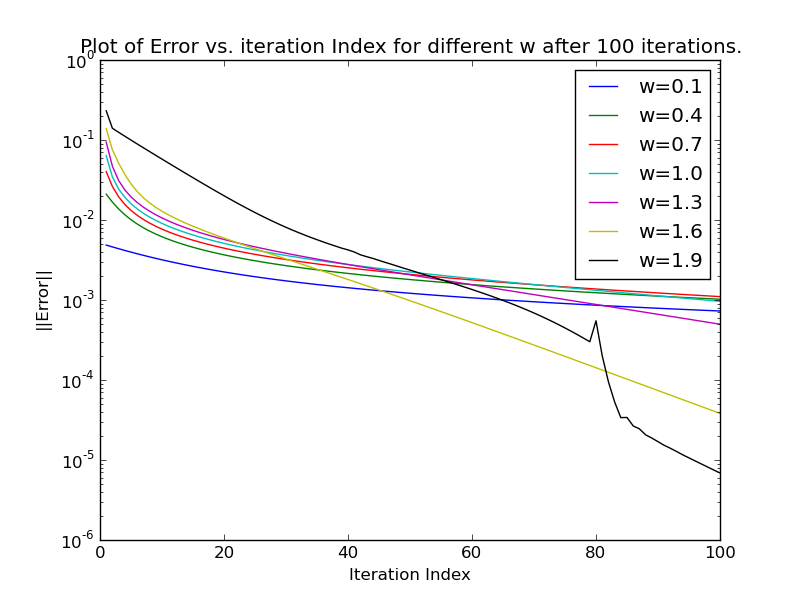
\includegraphics[width=10cm]{all_w_41_100_10.png}
\caption{Plot of norm of error vs. number of iterations for different w in SOR scheme for a 41x41 grid.}
\label{figure:}
\end{figure}

\begin{figure}[H] \label{figure}
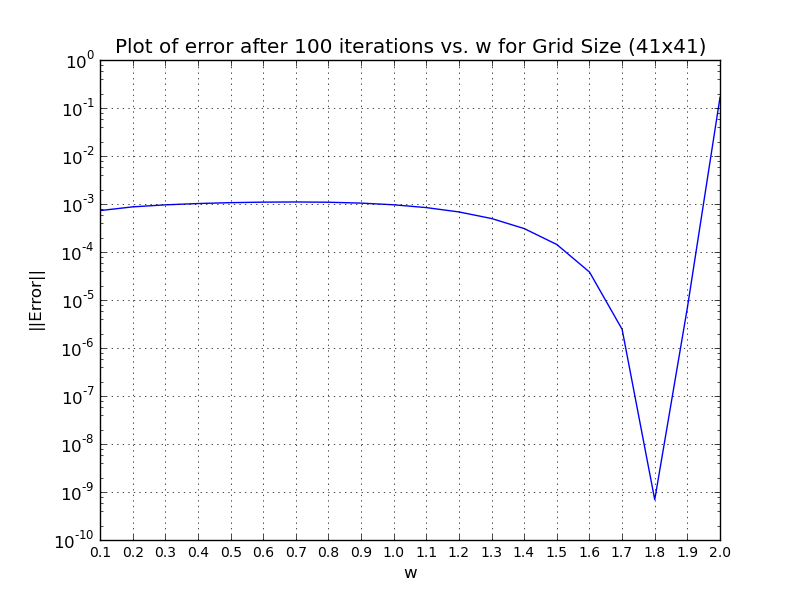
\includegraphics[width=10cm]{w_41_100_10.png}
\caption{Plot of norm of error at the end of 100 iterations vs. w in SOR scheme for a 41x41 grid.}
\label{figure:}
\end{figure}

\begin{description}
\item[]Plot changes.
\item[]Minimum error for 41x41 grid occurs at 1.8 after both 50 and 100 iterations, while minimum error occured at 0.1 after 10 iterations for the reason explained in Question 2.
\item[]The results obtained from error vs. w plot are in accordance with the residue vs. w plot.
\item[]Initially the error is high for high w values but decreases significantly after some iterations.
\end{description}

\newpage
\textbf{4. Once an approximate w\_opt is found, hunt for a better estimate for the optimal in the range, (w\_opt - 0.1, w\_opt + 0.1) with steps of w in $0.01$. Use 50 iterations.}

\begin{figure}[H] \label{figure}
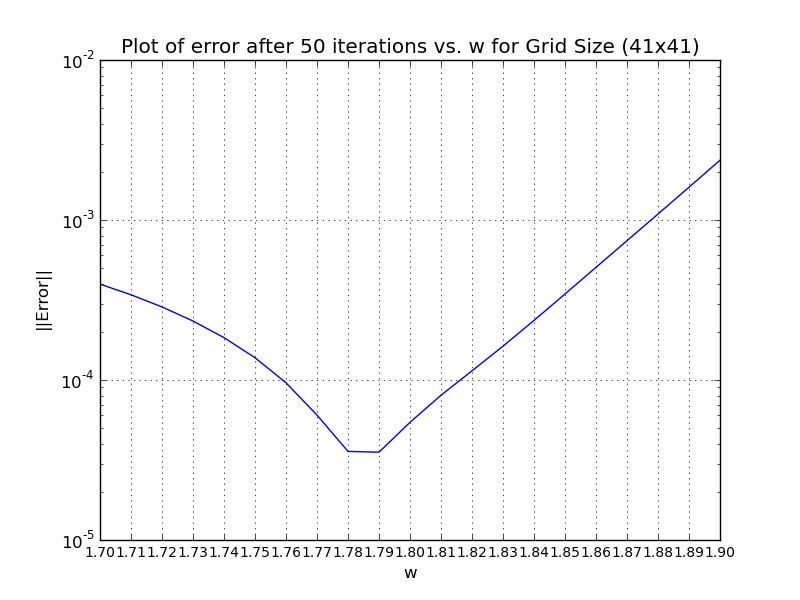
\includegraphics[width=10cm]{w_41_50_1.png}
\caption{Plot of norm of error at the end of 50 iterations vs. w in SOR scheme for a 41x41 grid.}
\label{figure:}
\end{figure}

\begin{description}
\item[]Minimum occurs somewhere between w = 1.78 and w = 1.79. A more exact value of w for which minimum error occurs can be hunt for by searching in the region 1.78 to 1.80 with resolution of 0.001 and so on.

\end{description}
\newpage
\textbf{5. Does the w\_opt change if N=101 and with a total of 100 iterations.}

\begin{figure}[H] \label{figure}
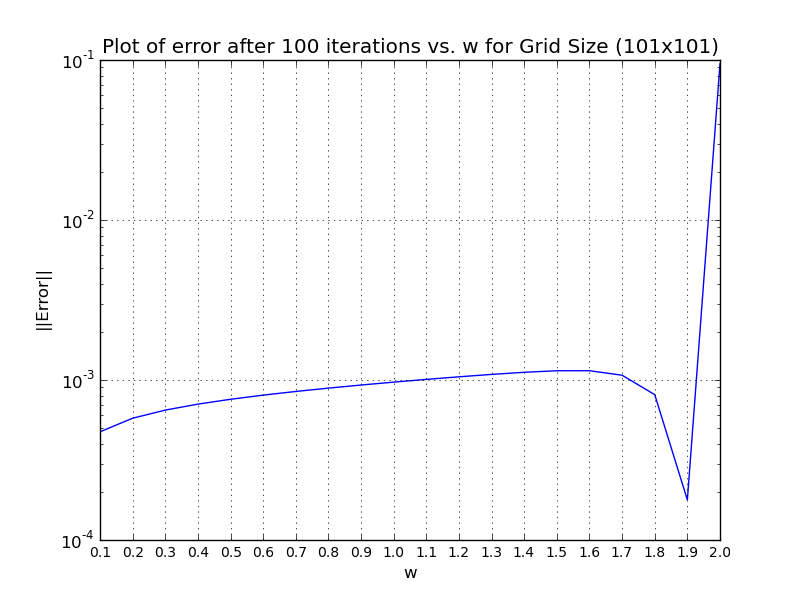
\includegraphics[width=10cm]{w_101_100_10.png}
\caption{Plot of norm of error at the end of 100 iterations vs. w (0,2)  in SOR scheme for a 101x101 grid .}
\label{figure:}
\end{figure}

\begin{figure}[H] \label{figure}
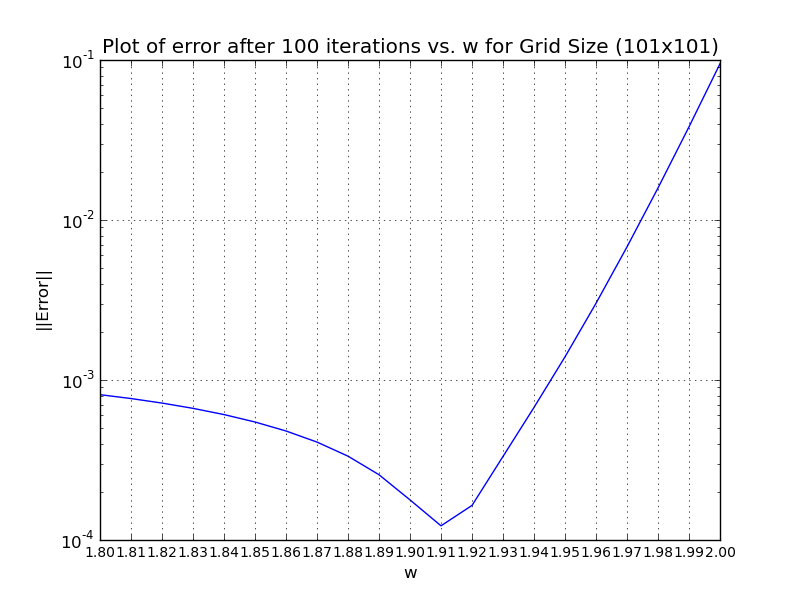
\includegraphics[width=10cm]{w_101_100_1.png}
\caption{Plot of norm of error at the end of 100 iterations vs. w (w\_opt - 0.1, w\_opt+0.1)in SOR scheme for a 101x101 grid.}
\label{figure:}
\end{figure}

\begin{figure}[H] \label{figure}
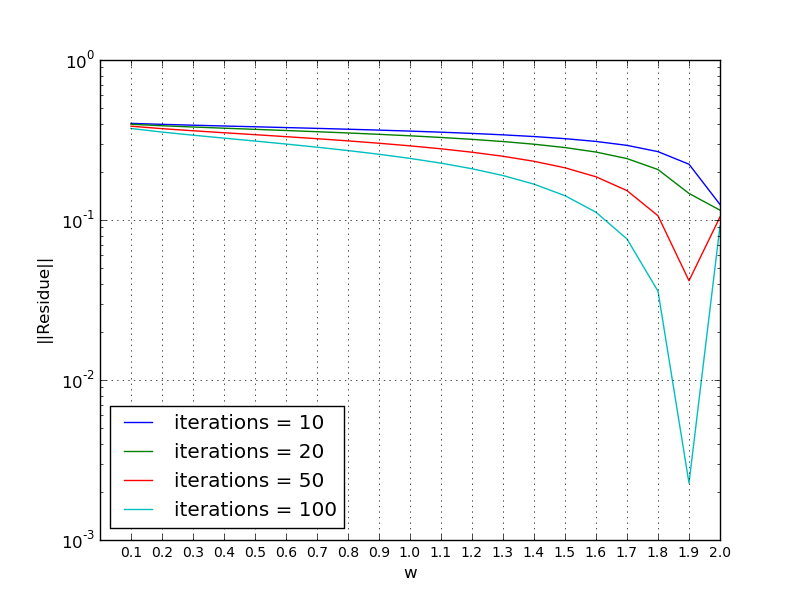
\includegraphics[width=10cm]{residue_101.png}
\caption{Plot of residue at the end of 10,20,50,100 iterations vs. w in SOR scheme for a 101x101 grid.}
\label{figure:}
\end{figure}

\begin{description}
\item[]Optimal w in SOR scheme for a 101x101 grid is close to 1.91 as evident from both error and residue plots.
\item[]As size of grid increases, optimal value of w increases.
\item[]From the residue vs. w plot, residue decreases continuously from 0.1 to around 1.9, but error increases first and then decreases till around 1.9. This happens because of the reason mentioned in Question 2.

\end{description}

\newpage
\textbf{6. Repeat the hunt for an optimal w\_opt (with w = linspace(1, 2, 11)) but this time calculate the number of iterations it takes to converge to machine epsilon instead of the error.  Plot the number of iterations vs. w.}

\begin{figure}[H] \label{figure}
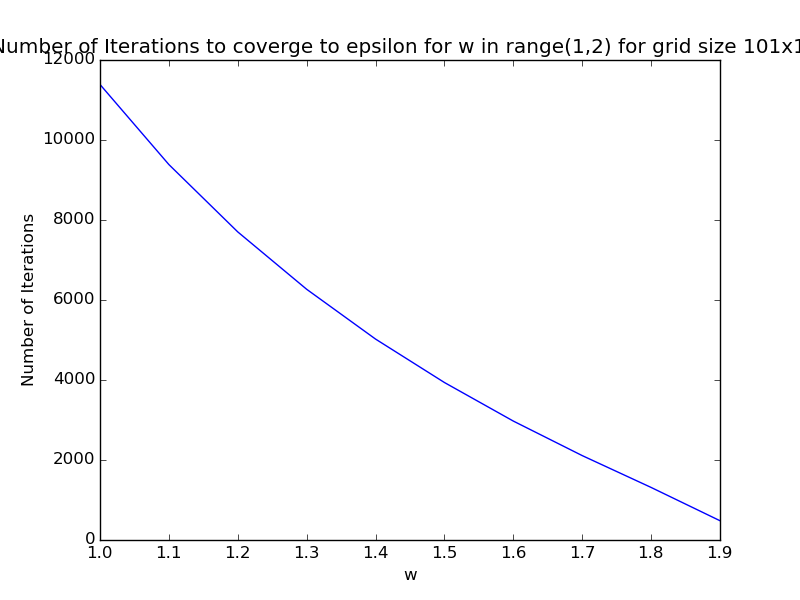
\includegraphics[width=10cm]{n_w_101.png}
\caption{Plot of number of iterations vs. w in SOR scheme for a 101x101 grid.}
\label{figure:}
\end{figure}

\begin{description}
\item[]Error continuously decreases with w from 1.0 to 1.9 for 101x101 grid.
\item[]Convergence is fastest (least number of iterations) occur for w = 1.9, which is in accordance with result obtained by hunting w after 100 iterations for 101x101 grid. 
\item[]For w = 2.0, iterations never converge.

\end{description}

\newpage
\textbf{7. Having found the optimal w, take N=101 and solve this using all the three schemes and plot the error versus the number of iterations in a semi-log plot.}

\begin{figure}[H] \label{figure}
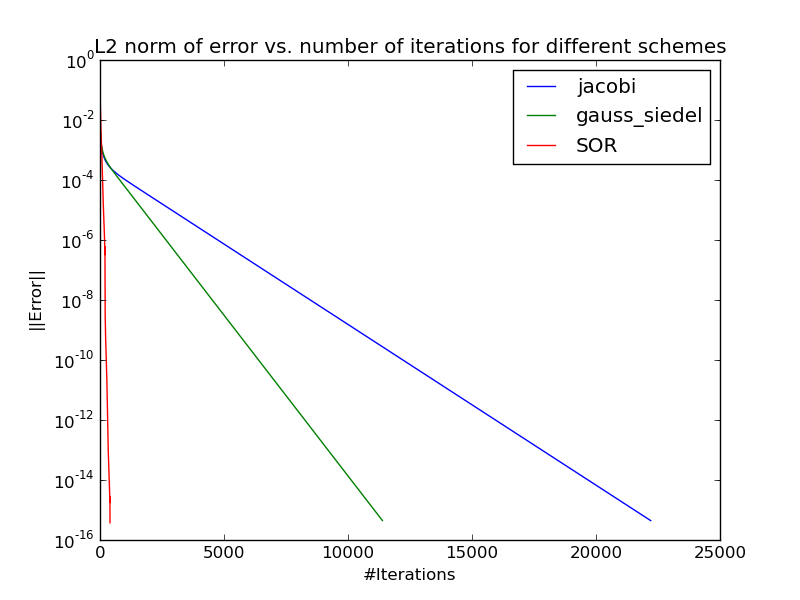
\includegraphics[width=10cm]{all_scheme_101_.png}
\caption{Plot of error vs. number of iterations till the convergence to machine\_epsilon for different schemes.}
\label{figure:}
\end{figure}

\begin{description}
\item[]Number of iterations taken to converge to machine\_epsilon for a 101x101 grid is least for $SOR (optimal\_w = 1.91) < Gauss Siedel < Jacobi Method$.
\item[]Slope for Gauss Siedel method is twice that of Jacobi method. Thus, Gauss siedel is twice as fast as Jacobi method.
\end{description}
\end{document}
